\documentclass{X:/Documents/Coding/Latex/myassignment}
%%Document info
\title{OFN Assignment 4}
\begin{document}
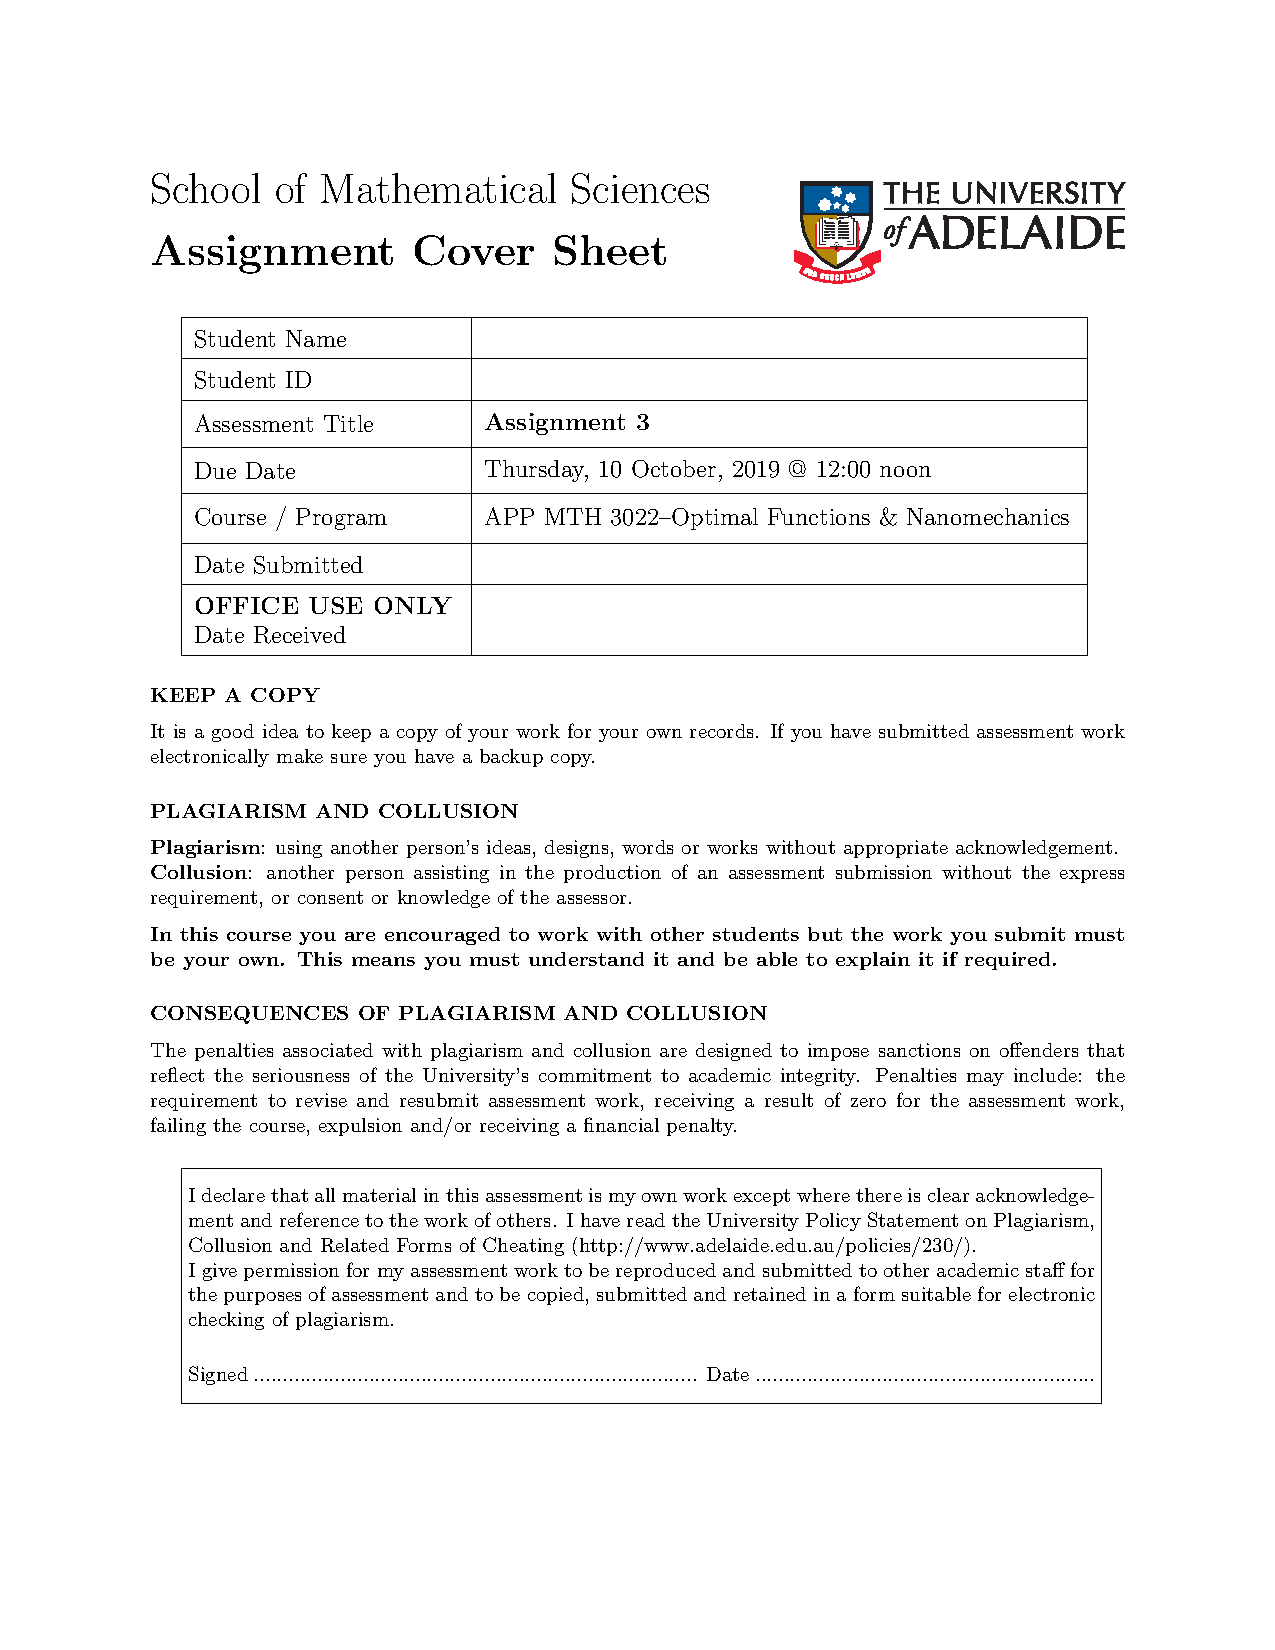
\includepdf{cover4}
\maketitle

\begin{enumerate}
%1
\item 
\begin{enumerate}
	%1a
	\item $dA$ is obtained using the cross product of the tangent vectors of the parametrisation
	\begin{align*}
		\dd r\theta &= \left(-b\sin\theta \sin\phi, b\cos\theta\sin\phi,0\right)\\
		\dd r\phi &= \left(b\cos\theta\cos\phi, b\sin\theta\cos\phi,-c\sin\phi\right)
	\end{align*}

	\[dA = \left|\dd r\theta \times \dd r\phi \right| d\theta d\phi\]
	\[\dd r\theta \times \dd r\phi= \begin{vmatrix}
		\vec i & \vec j & \vec k \\
		-b\sin\theta \sin\phi& b\cos\theta\sin\phi&0\\
		b\cos\theta\cos\phi& b\sin\theta\cos\phi&-c\sin\phi
	\end{vmatrix}\]
	\begin{align*}
		&= \left(-bc\cos\theta\sin^2\phi, bc\sin\theta\sin^2\phi, -b^2\sin^2\theta\sin\phi\cos\phi - b^2\cos\theta^2\sin\phi\cos\phi\right)\\
		&=\left(-bc\cos\theta\sin^2\phi, bc\sin\theta\sin^2\phi, -b^2\sin\phi\cos\phi\right) \\
		&= b\sin\phi\left(-c\cos\theta\sin\phi, c\sin\theta\sin\phi, -b\cos\phi\right) 
	\end{align*}
	\begin{align*}
		dA &= b\sin\phi\sqrt{(-c\cos\theta\sin\phi)^2 + (c\sin\theta\sin\phi)^2 + (-b\cos\phi)^2} d\theta d\phi\\
		&= b\sin\phi\sqrt{c^2\cos^2\theta\sin^2\phi + c^2\sin^2\theta\sin^2\phi + b^2\cos^2\phi} d\theta d\phi\\
		&= b\sin\phi\sqrt{c^2\sin^2\phi + b^2\cos^2\phi} d\theta d\phi\\
		&= b\sin^2\phi\sqrt{c^2-b^2} d\theta d\phi\\
	\end{align*}
	%1b
	\item 
	%1c
	\item 
\end{enumerate}

%question 2
\item 
\begin{enumerate}
	%2a
	\item 
	%2b
	\item 
\end{enumerate}
%question 3
\item 
\end{enumerate}


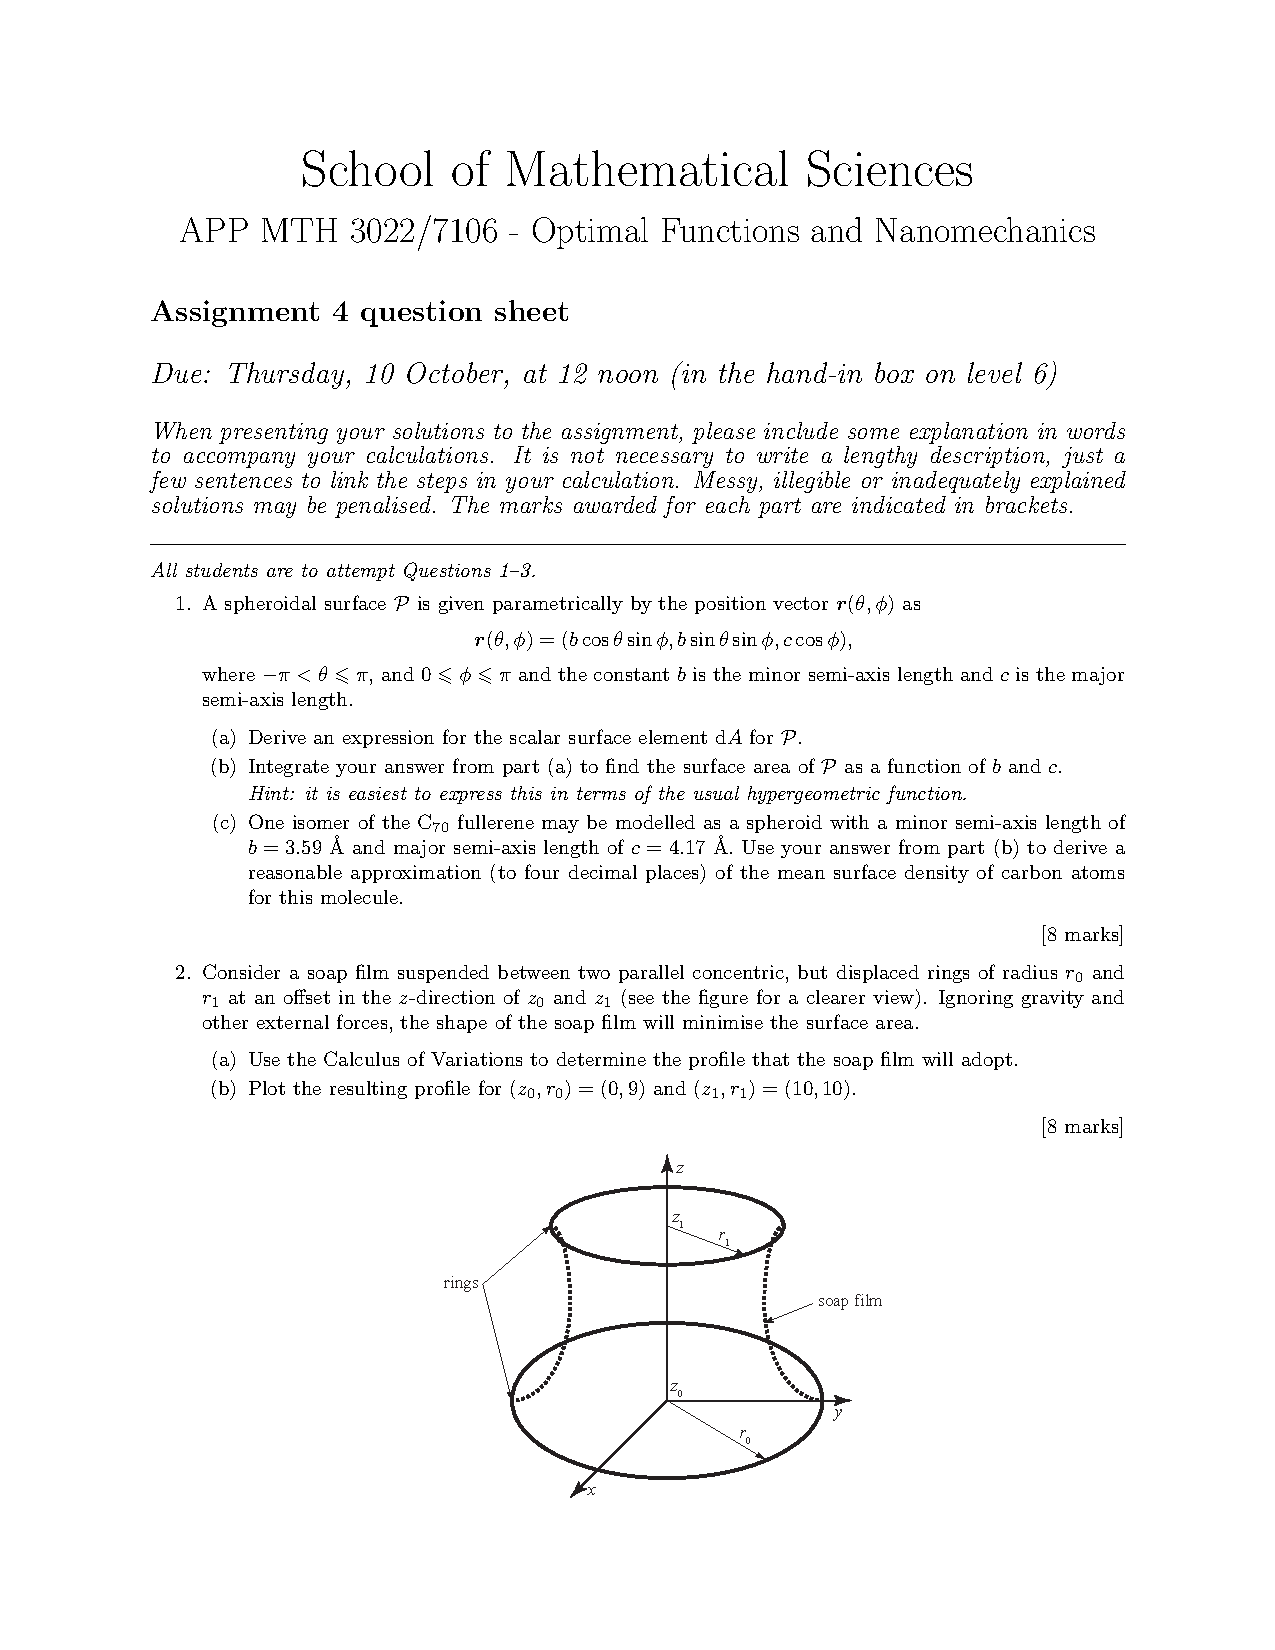
\includepdf[pages=1-]{assign4.pdf}

\end{document}